\usepgflibrary{shapes.misc}
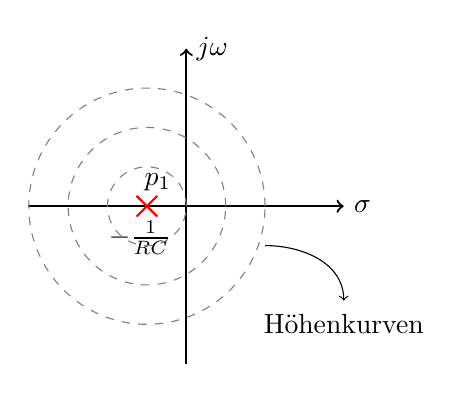
\begin{tikzpicture}
\begin{scope}[thick, ->]
  \draw (-2,0) -- +(4,0) node[right] {$\sigma$};
  \draw (0,-2) -- +(0,4) node[right] {$j \omega$};
\end{scope}
 
  \node[cross out, draw=red, thick] at (-0.5,0) {}
     node[below left=2] {$- \frac{1}{RC}$}
     node[above left=2] {$p_1$};

\draw[dashed, color=gray](-0.5,0) circle (1);
\draw[dashed, color=gray](-0.5,0) circle (0.5);
\draw[dashed, color=gray](-0.5,0) circle (1.5);
\draw (1,-0.5) edge[out=0, in=90, ->] (2,-1.2);
\node at (2,-1.5) {Höhenkurven};

\end{tikzpicture}